\chapter{Kiến thức nền tảng}
\label{Chapter2}
\graphicspath{{Chapter2/Chapter2Figs}}

\textit{Tong chương này, đầu tiên chúng tôi sẽ trình bày về mô hình 
``Auto-Encoders'', một mạng nơ-ron được dùng để học đặc trưng ẩn dựa trên
phương pháp học không giám sát.
Sau đó, chúng tôi giới thiệu và trình bày về nền tảng xác suất 
của ``Variational Auto-encoders'' (VAEs) và lợi ích mang lại của 
mô hình này so với ``Auto-Encoder'' trong tác vụ học đặc trưng ẩn; 
Những điểm lợi này chính là lý do mà chúng tôi tập trung nghiên cứu VAEs. 
Bên cạnh đó, chúng tôi sẽ trình bày về ``Maximum Likelihood Estimation'', 
một phương pháp dùng để đánh giá các tham số của mô hình, đại diện cho các tham số 
của các phân phối xác suất dựa trên dữ liệu huấn luyện. 
Chương này đặc biệt là phần về ``Variational Auto-Encoders'' 
cung cấp những kiến thức nền tảng để có thể hiểu rõ về những đề xuất 
của chúng tôi ở chương kế tiếp.}


% \textit{Bên cạnh đó, chúng tôi sẽ trình bày về ``Log-likelihood fuctions'' - 
% là phép đo mức độ học của mô hình dựa trên các dữ liệu ta quan sát được 
% cũng như các lựa chọn Log-likelihood fucntion cho các bài toán học máy hiện nay.}
% 7->10; 15->20; 15->20; 10->15; 2 (~60)
\newpage

\section{Mô hình rút trích đặc trưng ``Auto-Encoder''}
\label{chap2/sec1}
Mô hình ``Auto-Encoder'' là một mạng nơ-ron truyền thẳng được huấn luyện
để cố gắng sao chép đầu vào của nó thành đầu ra. Bên trong ``Auto-Encoder''
có một lớp ẩn \textbf{\textit{h}} mô tả đặc trưng ẩn, gọi là véc-tơ biểu diễn ẩn đại diện cho đầu vào của nó.

Kiến trúc của một ``Auto-Encoder'' (được minh họa trong hình~\ref{fig_AE}) bao gồm hai phần:
\begin{itemize}
    \item Bộ mã hóa (encoder) ánh xạ véc-tơ đầu vào sang véc-tơ biểu diễn ẩn: 
    \begin{center}
        \begin{math}
            \centering
            \textbf{\textit{h}} = f(x)
        \end{math} 
            
    \end{center}
    \item Bộ giải mã (decoder) có nhiệm vụ cố gắng tái tạo lại véc-tơ đầu vào từ véc-tơ biểu diễn ẩn:
    \begin{center}
        \begin{math}
            \hat{x} = g(\textbf{\textit{h}}) = g(f(x))
        \end{math}
    \end{center}
\end{itemize}


\begin{figure}
    \centering
	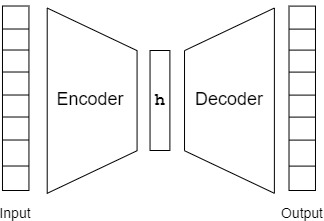
\includegraphics[width=0.6\textwidth]{AE.jpg}
    \caption{Minh họa ``Auto-Encoder''}
    \label{fig_AE}
\end{figure}

``Auto-Encoder'' được huấn luyện bằng cách cực tiểu hóa hàm lỗi là độ sai lệch giữa dữ liệu được tái tạo
với dữ liệu đầu vào. 
\begin{equation}
\label{AE_loss}
    L(x, g(f(x)))
\end{equation}
Các hàm để tính độ lỗi thường được dùng là ``Mean-square error'' hoặc ``Binary cross-entropy''.
Tương tự như các mạng nơ-ron khác, ``Auto-Encoder'' có thể được huấn luyện bằng phương pháp ``Gradient-descent''
với thuật toán lan truyền ngược (``back-propagation'').

Khi thiết kế mô hình, kiến trúc của encoder, decoder
và kích thước của véc-tơ \textbf{\textit{h}} được xem như những siêu tham số của mô hình.
Bằng các cách thiết lập khác nhau, mô hình sẽ có những tính chất khác nhau. 
``Auto-Encoder'' với encoder và decoder là những hàm phi tuyến (cụ thể là mạng nơ-ron với hàm kích hoạt phi tuyến)
với khả năng tính toán quá mạnh hay trường hợp kích thước của véc-tơ \textbf{\textit{h}}
lớn hơn hoặc bằng so với véc-tơ đầu vào sẽ dẫn đến mô hình chỉ học cách sao chép thay vì trích xuất các đặc trưng ẩn từ dữ liệu. 

Thông thường, một ``Auto-Encoder'' sao chép một cách ``hoàn hảo'' đầu vào thành đầu ra
sẽ không có nhiều ý nghĩa. Thay vào đó, ``Auto-Encoder'' được thiết kế với các ràng buộc để không thể
học cách sao chép ``hoàn hảo'' mà chỉ có thể sao chép gần đúng, từ đó ta hy vọng quá trình 
huấn luyện ``Auto-Encoder'' sẽ thu được véc-tơ biểu diễn ẩn có những thông tin hữu ích.

Từ véc-tơ biểu diễn ẩn thu được trong quá trình huấn luyện ``Auto-Encoder'', ta có thể áp dụng mô hình này
như một mô hình trích xuất đặc trưng ẩn từ dữ liệu, làm đầu vào cho các tác vụ khác. 
Hoặc véc-tơ biểu diễn ẩn này có thể áp dụng được trong các tác vụ giảm chiều dữ liệu hỗ trợ cho các tác vụ
lưu trữ, truy vấn, tìm kiếm.

    \subsection{``Undercomplete Auto-Encoder''}
    \label{chap2/subsec11}
    Như đã trình bày trước đó, việc sao chép đầu vào thành đầu ra của ``Auto-Encoder'' không mang nhiều ý nghĩa.
    Ta cần các ràng buộc để có được \textbf{\textit{h}}
    nhận các thuộc tính hữu ích với các ràng buộc khi thiết kế mô hình.
    
    Một cách ràng buộc để mô hình có thể học được các đặc trưng ẩn từ dữ liệu
    là giới hạn véc-tơ đặc trưng ẩn \textbf{\textit{h}} có kích thước nhỏ hơn đáng kể so với véc-tơ đầu vào;
    tính chất này được gọi là ``under-complete''.
    
    Mô hình ``Auto-Encoder'' với kích thước \textbf{\textit{h}} nhỏ hơn đáng kể so với kích thước của véc-tơ đầu vào
    được gọi là ``Undercomplete Auto-Encoder''. Việc giới hạn này sẽ buộc mô hình phải nắm bắt các đặc trưng
    nổi bật nhất.

    Quá trình huấn luyện ``Undercomplete Auto-Encoder'' cũng giống với mô hình ``Auto-Encoder'',
    ta cần cực tiểu hóa hàm lỗi (công~thức~\ref{AE_loss}) là độ sai lệch giữa dữ liệu được tái tạo
    với dữ liệu đầu vào.

    ``Undercomplete Auto-Encoder'' là mô hình tốt để sử dụng cho các tác vụ tiêu biểu của ``Auto-Encoder'' truyền thống
    như trích xuất đặc trưng, giảm chiều dữ liệu 
    bởi vì tính chất ``under-complete'' của mô hình giúp dễ dàng thu được véc-tơ biểu diễn ẩn mang những thông tin hữu ích.


    \subsection{``Denoising Auto-Encoder''}
    \label{chap2/subsec12}
    
    Hàm lỗi của một ``Auto-Encoder'' thông thường sẽ ``phạt'' một mức nhất định với các mẫu dữ liệu được tái tạo lại
    khác với dữ liệu đầu vào. Điều này vô hình chung khuyến khích 
    nghĩa là 
    \begin{math}
        f \circ g
    \end{math}
    là một hàm đồng nhất nếu khả năng tính toán của 
    \begin{math}
        f
    \end{math} 
    và
    \begin{math}
        g
    \end{math}
    cho phép. Nói đơn giản hơn, điều này là việc mô hình sao chép ``hoàn hảo'' đầu vào thành đầu ra của nó.
    Khi đó, véc-tơ biểu diễn ẩn sẽ không có các thông tin hữu ích. 

    Bằng cách thay đổi cách tính toán độ lỗi khi tái tạo lại, cụ thể là thêm nhiễu vào véc-tơ đầu vào, 
    sau đó tính toán độ lỗi là đầu ra được mô hình tái tạo lại so với đầu vào ban đầu như sau:
    \begin{equation}
        L(x, g(f(\tilde{x})))
    \end{equation}
    với 
    \begin{math} \tilde{x} \end{math}
    là véc-tơ đầu vào 
    \begin{math}
        x
    \end{math} 
    được thêm một độ nhiễu, ta có được mô hình ``Denoising Auto-Encoder'' (hình~\ref{fig_DAE}). 
    \begin{figure}
        \centering
        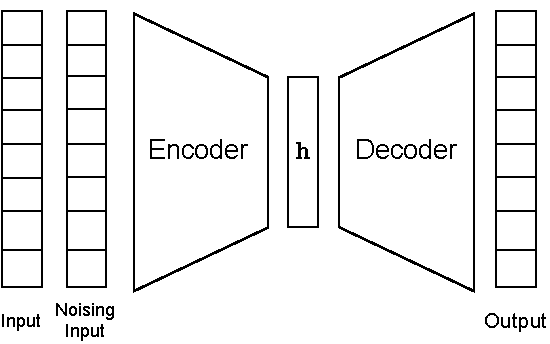
\includegraphics{DAE.pdf}
        \caption{Minh họa ``Denoising Auto-Encoder''}
        \label{fig_DAE}
    \end{figure}
    
    ``Denoising Auto-Encoder'' phải học cách khử độ nhiễu đã được thêm vào véc-tơ đầu vào,
    giảm khả năng sao chép của mô hình.






\section{``Variational Auto-Encoder''} \label{chap2/sec2}
    \subsection{Nền tảng xác suất} \label{chap2/subsec21}
        \subsubsection{ ``Maximum Likelihood Estimation''}
    \subsection{Phương pháp ``Variational Inference'' } \label{chap2/subsec22}
    \subsection{Độ sai biệt ``Kullback-Leiber Devergence'' giữa hai phân phối xác suất}  \label{chap2/subsec23}